% %
% cooperation_manual.TEX 
% based on ?
% NEOSTEL documentation
% Prepared by Piotr Zdunek, Paweł Zienkiewicz, Jacek Kołodziejski and Łukasz Kociszewski
%  Creotech Instruments S.A.
%
\documentclass[twoside,a4paper]{refart}
%\usepackage{makeidx}
\usepackage[utf8]{inputenc}
\usepackage{imakeidx}
\usepackage{ifthen}
\usepackage[]{graphicx}
\usepackage{amsmath}
\usepackage{amsfonts}
\usepackage{amssymb}
\usepackage{url}
\usepackage{hyperref}
\hypersetup{
    colorlinks,
    citecolor=black,
    filecolor=black,
    linkcolor=black,
    urlcolor=black
}
\sloppy
%\usepackage[acronym,toc]{glossaries}
%\loadglsentries[\acronymtype]{cooperation_glossary}
%\usepackage[acronym]{glossaries} %http://en.wikibooks.org/wiki/LaTeX/Glossary

%%%%%%%%%%%%%%%%%%%%%%%%%%%%ADDED PACKAGES%%%%%%%%%%%%%%%%%%%%%%%%%%%%%%%%%%%
\usepackage{epsf}
\usepackage{epstopdf}


% or using \input:
%\input{INP-00-glossary}




\def\bs{\char'134 } % backslash in \tt font.
\newcommand{\ie}{i.\,e.,}
\newcommand{\eg}{e.\,g..}
\DeclareRobustCommand\cs[1]{\texttt{\char`\\#1}}

\title{Neostel Zynq Coop Manual}
\author{Paweł Zienkiewicz\\
Piotr Zdunek \\
Łukasz Kociszewski \\
Jacek Kołodziejski}

\date{}
\emergencystretch1em  %

\pagestyle{myfootings}
\markboth{Neostel Zynq Coop Manual}%
         {Neostel Zynq Coop Manual}

\makeindex 

\setcounter{tocdepth}{2}
%\makeglossaries

\begin{document}
%\include{cooperation_glossary}

\maketitle

\begin{abstract}
        This document describes methods used in FPGA/ARM Zynq Neostel development.
\end{abstract}

%%%%%%%%%%%%%%%%%%%%%%%%%%%%%%%%%%%%%%%%%%%%%%%%%%%%%%%%%%%%%%%%%%%%%%
\tableofcontents

\newpage
%%%%%%%%%%%%%%%%%%%%%%%%%%%%%%%%%%%%%%%%%%%%%%%%%%%%%%%%%%%%%%%%%%%%%%
\section{Glossary} 
\input{tex/cooperation_glossary.tex}
\newpage
%%%%%%%%%%%%%%%%%%%%%%%%%%%%%%%%%%%%%%%%%%%%%%%%%%%%%%%%%%%%%%%%%%%%%%
\section{Specification}
\subsection{Software}
\subsection{OS}

\cite{ART:MENTOR_OS}

\subsection{HDL}
\subsection{?}


\begin{itemize}
\item Linux runs on one ARM Core (CPU0) \cite{XilinxZynqWiki}
\item Baremetal application runs on CPU1 (it is handling exceptions from PL)
\item PTP timestamp is being placed in OCM memory
\item CCD driver is made in PL 
\item Shutter driver is made in PL
\item Network boot for Zynq with u-boot bootscript for failsafe \cite{TIWikiUBoot,UbootParsing}
\item Network boot with read only FS via NFS?
\item Archive on remote attached storage
\item Failsafe of Linux OS?
\end{itemize}

\newpage
%%%%%%%%%%%%%%%%%%%%%%%%%%%%%%%%%%%%%%%%%%%%%%%%%%%%%%%%%%%%%%%%%%%%%%
\section{Technical assumptions}

\subsection{Booting diagram}

\begin{figure}[!htb]
%\begin{center}
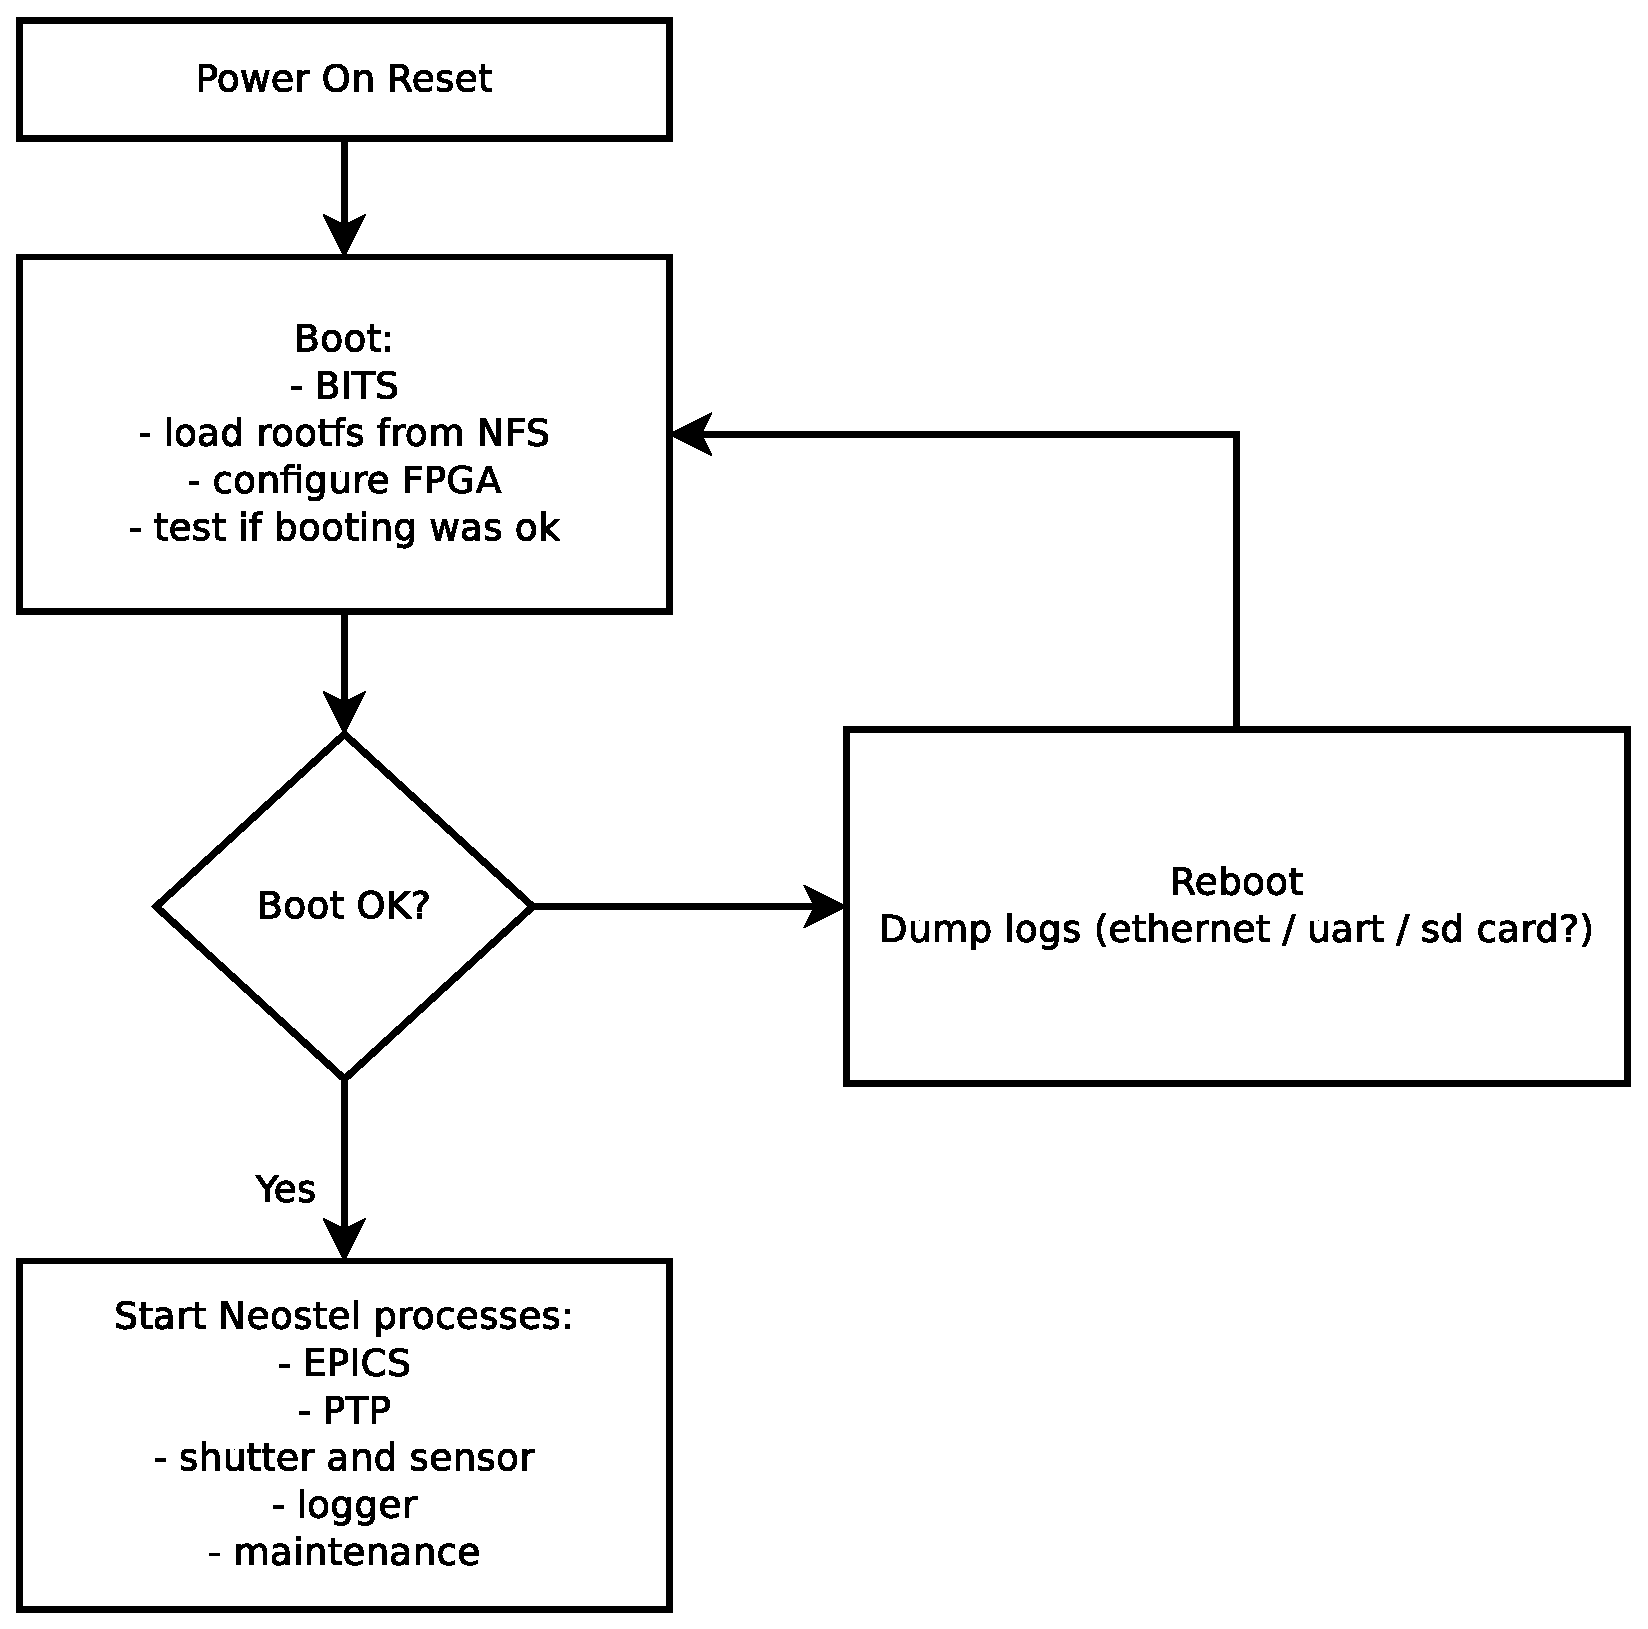
\includegraphics[scale=.35]{img/general.eps}

\caption{General boot flowchart}
%\end{center}
%todo center caption
\label{fig:digraph}
\end{figure}


\subsection{Failsafe reporting specification}

How will the system report error on following cases? 
What needs to be solved is how will reporting be done before linux boots.
There can be a system checker IP in logic but it doesn't check e.g. power suppiles. Such an IP can generate heartbit. 

Assumptions:
\begin{itemize}
\item It is assumed that device is powered properly and all of the power lines
are ok.
\end{itemize}

Interfaces for reporting errors:
\begin{itemize}
\item RS485
\item Ethernet

\end{itemize}

TO DO
\begin{itemize}
\item Learn how does the Zynq Watchdog works. 
\end{itemize}


\newpage
%%%%%%%%%%%%%%%%%%%%%%%%%%%%%%%%%%%%%%%%%%%%%%%%%%%%%%%%%%%%%%%%%%%%%%
\section{Hardware platform details}

\newpage
%%%%%%%%%%%%%%%%%%%%%%%%%%%%%%%%%%%%%%%%%%%%%%%%%%%%%%%%%%%%%%%%%%%%%%
\section{Development platform (and software) details}


\newpage
%%%%%%%%%%%%%%%%%%%%%%%%%%%%%%%%%%%%%%%%%%%%%%%%%%%%%%%%%%%%%%%%%%%%%%
\section{Boot Process}

\begin{figure}[!htb]
%\begin{center}
\includegraphics[scale=.35]{img/boot2.eps}

\caption{Specific boot flowchart}
%\end{center}
%todo center caption
\label{fig:boot_graph}
\end{figure}

\newpage
%%%%%%%%%%%%%%%%%%%%%%%%%%%%%%%%%%%%%%%%%%%%%%%%%%%%%%%%%%%%%%%%%%%%%%
\section{Linux OS details}


\newpage
%%%%%%%%%%%%%%%%%%%%%%%%%%%%%%%%%%%%%%%%%%%%%%%%%%%%%%%%%%%%%%%%%%%%%%
\section{Linux OS startup}


\newpage
%%%%%%%%%%%%%%%%%%%%%%%%%%%%%%%%%%%%%%%%%%%%%%%%%%%%%%%%%%%%%%%%%%%%%%
\section{Bare Metal software details}


\newpage
%%%%%%%%%%%%%%%%%%%%%%%%%%%%%%%%%%%%%%%%%%%%%%%%%%%%%%%%%%%%%%%%%%%%%%
\section{BM-Linux-FPGA cooperation}


\newpage
%%%%%%%%%%%%%%%%%%%%%%%%%%%%%%%%%%%%%%%%%%%%%%%%%%%%%%%%%%%%%%%%%%%%%%
\section{PTP time synchronisation}


\newpage
%%%%%%%%%%%%%%%%%%%%%%%%%%%%%%%%%%%%%%%%%%%%%%%%%%%%%%%%%%%%%%%%%%%%%%
\section{Interfacing capabilities and limitations}


\newpage
%%%%%%%%%%%%%%%%%%%%%%%%%%%%%%%%%%%%%%%%%%%%%%%%%%%%%%%%%%%%%%%%%%%%%%
\section{Interfacing with remote systems}


\newpage

%%%%%%%%%%%%%%%%%%%%%%%%%%%%%%%%%%%%%%%%%%%%%%%%%%%%%%%%%%%%%%%%%%%%%%
\section{Known problems}


\newpage
%%%%%%%%%%%%%%%%%%%%%%%%%%%%%%%%%%%%%%%%%%%%%%%%%%%%%%%%%%%%%%%%%%%%%%
\printindex
\bibliography{cooperation_manual}   %>>>> bibliography data in cooperation_manual.bib
\bibliographystyle{amsplain}



\end{document}
